\documentclass{beamer}
\usepackage{fontspec}
\setsansfont[Path=C:/Users/User/AppData/Local/Microsoft/Windows/Fonts/,UprightFont=Helvetica.ttf,BoldFont=Helvetica-Bold.ttf,ItalicFont=Helvetica-Oblique.ttf,BoldItalicFont=Helvetica-BoldOblique.ttf]{Helvetica.ttf}
\usetheme{Berlin}
\usefonttheme[onlymath]{serif}
\setbeamertemplate{footline}{%
  \leavevmode%
  \hbox{%
  \begin{beamercolorbox}[wd=.88\paperwidth,ht=2.6ex,dp=1.1ex,leftskip=1.2em]{author in head/foot}%
    \ifodd\insertframenumber\relax
      \scriptsize An Automatic Following/Forming Framework for Inverter-Based Resources%
    \else
      \scriptsize Department of Electrical Engineering, School of Engineering, KMITL%
    \fi
  \end{beamercolorbox}%
  \begin{beamercolorbox}[wd=.12\paperwidth,ht=2.6ex,dp=1.1ex,center]{date in head/foot}%
    \scriptsize \insertframenumber/\inserttotalframenumber
  \end{beamercolorbox}}%
}

\usepackage{xcolor}
\usepackage{graphicx}
\usepackage{amsmath,amsfonts,amssymb}
\usepackage{bm}
\setcounter{MaxMatrixCols}{20}
\usepackage{booktabs,array,multicol}
\usepackage{tikz}
\usetikzlibrary{arrows.meta,positioning,shapes}

\definecolor{myblue}{rgb}{0.0,0.0,0.7}
\definecolor{pnavy}{HTML}{0F2A4A}
\definecolor{pblue}{HTML}{1D5288}
\definecolor{pgreen}{HTML}{1E7E34}
\definecolor{pred}{HTML}{A93226}
\definecolor{pyellow}{HTML}{B7950B}
\setbeamercolor{item}{fg=myblue}
\setbeamercolor{block title}{bg=myblue,fg=white}
\setbeamercolor{block body}{bg=blue!7,fg=black}
\setbeamercolor{itemize item}{fg=myblue}
\setbeamercolor{custom top bar}{bg=black,fg=white}
\setbeamercolor{custom sub bar}{bg=myblue,fg=white}
\setbeamertemplate{navigation symbols}{}
\setbeamercolor{frametitle}{bg=myblue!82!black,fg=white}
\setbeamertemplate{section in toc}[sections numbered]

\setbeamertemplate{background}{}
\setbeamertemplate{headline}{}

\title{\large\textbf{Project: An Automatic Following/Forming Framework\\for Inverter-Based Resources}}
\author{Mr. Phichitchai Jueajan (66010569)\\Mr. Pakkapol Phdungdan (66010612)\\[0.2cm]
Advisor: Dr. Tossaporn Surinkaew\\Co-advisor: Prof. Dr. Issarachai Ngamroo}
\institute{Department of Electrical Engineering, School of Engineering\\
King Mongkut's Institute of Technology Ladkrabang (KMITL)}
\date{}
\titlegraphic{}
\newcommand{\pu}{\,\mathrm{p.u.}}

\begin{document}

\begin{frame}[plain]
  \titlepage
\end{frame}

\begin{frame}{Table of Contents}
\centering
\renewcommand{\arraystretch}{1.65}
\begin{tabular}{c@{\hspace{0.35cm}}l}
\colorbox{myblue}{\makebox[0.52cm][c]{\color{white}\Large 1}} & {\Large Introduction and Motivation}\\
\colorbox{myblue}{\makebox[0.52cm][c]{\color{white}\Large 2}} & {\Large Project Objectives}\\
\colorbox{myblue}{\makebox[0.52cm][c]{\color{white}\Large 3}} & {\Large System Workflow and Case Study}\\
\colorbox{myblue}{\makebox[0.52cm][c]{\color{white}\Large 4}} & {\Large PF, SSSA and TS Formulation}\\
\colorbox{myblue}{\makebox[0.52cm][c]{\color{white}\Large 5}} & {\Large Dual-Mode IBR and Switching}\\
\colorbox{myblue}{\makebox[0.52cm][c]{\color{white}\Large 6}} & {\Large Results and Conclusions}
\end{tabular}
\end{frame}
\section{Introduction}
\begin{frame}{Introduction}
\begin{columns}[c,onlytextwidth]
\column{0.48\textwidth}
\small
\begin{block}{Grid-following (GFL)}
\begin{itemize}
  \item PLL-synchronized current control
  \item Requires an external voltage-angle reference
  \item Effective while a strong grid reference exists
\end{itemize}
\end{block}
\column{0.48\textwidth}
\small
\begin{block}{Grid-forming (GFM)}
\begin{itemize}
  \item Establishes voltage angle and frequency
  \item Supports weak-grid and islanded operation
  \item Can replace the lost reference after SG disconnection
\end{itemize}
\end{block}
\end{columns}
\end{frame}

\section{Objectives}
\begin{frame}{Project Objectives}
\small
\begin{enumerate}
  \item Develop one in-house analysis chain for \textbf{Power Flow}, \textbf{SSSA}, and \textbf{Time-Domain Simulation}.
  \item Model four converter resources with a common plant and selectable \textbf{GFL/GFM} controller branches.
  \item Determine admissible GFM configurations from the network condition instead of fixing the number of forming units in advance.
  \item Verify automatic mode transitions, island support, and SG reconnection under one disturbance chronology.
\end{enumerate}
\vspace{0.35cm}
\begin{block}{Scope}
IEEE 14-bus test system, one synchronous generator, four dual-mode IBRs, automatic reference support, and event-driven nonlinear simulation.
\end{block}
\end{frame}

\section{System Workflow}
\begin{frame}{Overall Analysis and Switching Workflow}
\centering
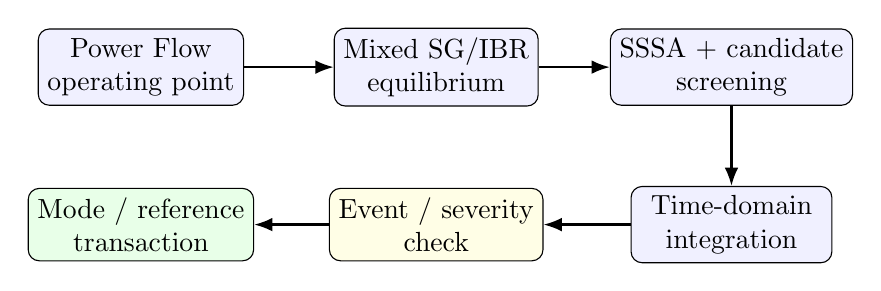
\begin{tikzpicture}[>=Latex,
  proc/.style={draw,rounded corners,minimum width=2.55cm,minimum height=0.80cm,align=center,fill=blue!6},
  check/.style={draw,rounded corners,minimum width=2.65cm,minimum height=0.80cm,align=center,fill=yellow!10},
  trans/.style={draw,rounded corners,minimum width=2.75cm,minimum height=0.80cm,align=center,fill=green!9}]
\node[proc] (pf) at (0,1.65) {Power Flow\\operating point};
\node[proc] (eq) at (3.75,1.65) {Mixed SG/IBR\\equilibrium};
\node[proc] (sssa) at (7.50,1.65) {SSSA + candidate\\screening};
\node[proc] (ts) at (7.50,-0.35) {Time-domain\\integration};
\node[check] (event) at (3.75,-0.35) {Event / severity\\check};
\node[trans] (sw) at (0,-0.35) {Mode / reference\\transaction};
\draw[->,thick] (pf)--(eq);
\draw[->,thick] (eq)--(sssa);
\draw[->,thick] (sssa)--(ts);
\draw[->,thick] (ts)--(event);
\draw[->,thick] (event)--(sw);
\end{tikzpicture}
\vspace{0.35cm}
\begin{block}{Runtime decision}
\footnotesize No trigger: advance to the next TS step. Triggered event: certify and commit the mode/reference transaction only after current continuity and right-limit KCL convergence.
\end{block}
\end{frame}


\section{Study System}
\begin{frame}{Case Study: IEEE 14-Bus with 1 SG + 4 Dual-Mode IBRs}
\begin{columns}[c,onlytextwidth]
\column{0.34\textwidth}
\footnotesize
\begin{block}{Resource mapping}
\begin{tabular}{lc}
\toprule
Resource & Bus \\
\midrule
SG1  & 1 \\
IBR1 & 2 \\
IBR2 & 3 \\
IBR3 & 6 \\
IBR4 & 8 \\
\bottomrule
\end{tabular}
\end{block}
\begin{itemize}
  \item SG1: normal synchronous reference
  \item IBR1--IBR4: dual-mode GFL/GFM converters
\end{itemize}
\column{0.62\textwidth}
\centering
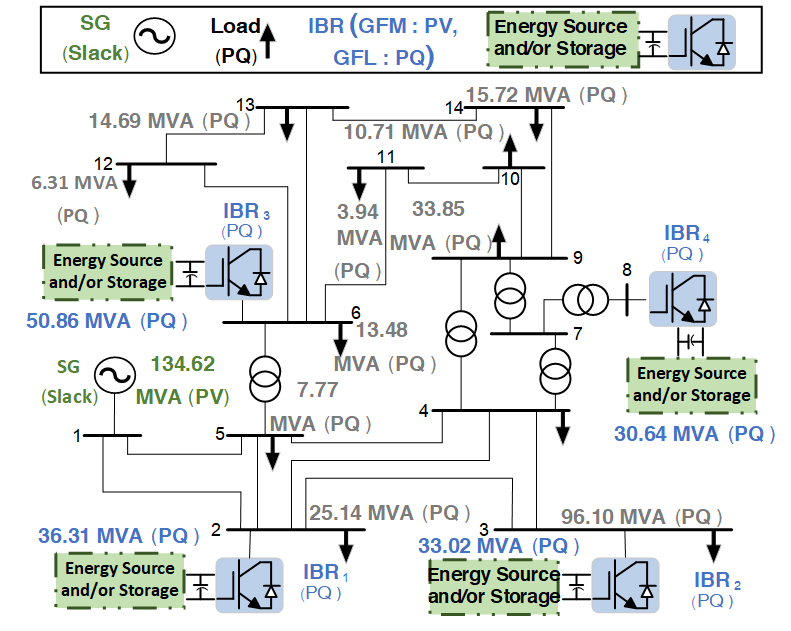
\includegraphics[width=0.98\linewidth]{figures/14 Bus kup.png}
\end{columns}
\end{frame}

\section{Power Flow}
\begin{frame}{Power Flow Formulation}
\begin{columns}[t,onlytextwidth]
\column{0.60\textwidth}
\scriptsize
Following the polar form used in Hadi Saadat,
\[
Y_{ik}=|Y_{ik}|\angle\theta_{ik},\qquad V_i=|V_i|\angle\delta_i
\]
\begin{align*}
P_i&=\sum_{k=1}^{n}|V_i||V_k||Y_{ik}|\cos(\theta_{ik}+\delta_k-\delta_i),\\
Q_i&=-\sum_{k=1}^{n}|V_i||V_k||Y_{ik}|\sin(\theta_{ik}+\delta_k-\delta_i).
\end{align*}
\column{0.35\textwidth}
\scriptsize
\begin{block}{Bus constraints}
\centering
\setlength{\tabcolsep}{3.5pt}
\begin{tabular}{lll}
\toprule
Type & Specified & Solved \\
\midrule
Slack & $|V|,\delta$ & $P,Q$ \\
PV & $P,|V|$ & $Q,\delta$ \\
PQ & $P,Q$ & $|V|,\delta$ \\
\bottomrule
\end{tabular}
\end{block}
\end{columns}
\vspace{0.10cm}
\scriptsize
\textbf{Newton--Raphson correction}
\[
\Delta P_i=P_i^{sch}-P_i,\qquad \Delta Q_i=Q_i^{sch}-Q_i
\]
\[
\boxed{\begin{bmatrix}\Delta\bm P\\\Delta\bm Q\end{bmatrix}
=\bm J_{PF}\begin{bmatrix}\Delta\bm\delta\\\Delta|\bm V|\end{bmatrix}}
\]
\[
\bm\delta^{(r+1)}=\bm\delta^{(r)}+\Delta\bm\delta^{(r)}
\]
\[
|\bm V|^{(r+1)}=|\bm V|^{(r)}+\Delta|\bm V|^{(r)}
\]
\end{frame}
\section{Small-Signal Stability}
\begin{frame}{Small-Signal Stability Analysis (SSSA)}
\begin{columns}[c,onlytextwidth]
\column{0.56\textwidth}
\small
\textbf{Linear small-signal model}
\[
\Delta\dot{\bm x}=\bm A\Delta\bm x+\bm B\Delta\bm u
\]
For the autonomous stability study used here, no AVR/PSS perturbation input is applied:
\[
\boxed{\Delta\dot{\bm x}=\bm A\Delta\bm x}
\]
The state matrix is obtained from the linearized DAE:
\[
\boxed{\bm A=\bm f_x-\bm f_y\left(\bm g_y\backslash\bm g_x\right)}
\]
\column{0.40\textwidth}
\small
\textbf{Modal analysis}
\[
\boxed{\bm A\bm\phi_i=\lambda_i\bm\phi_i}
\]
\[
\lambda_i=\sigma_i+j\omega_i,\qquad
f_i=\frac{|\omega_i|}{2\pi}
\]
\[
\zeta_i=-\frac{\sigma_i}{\sqrt{\sigma_i^2+\omega_i^2}}
\]
\begin{block}{Stability criterion}
$\operatorname{Re}(\lambda_i)<0$ for every physical mode, together with the declared damping-ratio floor.
\end{block}
\end{columns}
\end{frame}
\section{Time-Domain Simulation}
\begin{frame}{Time-Domain Simulation (TS)}
\begin{columns}[t,onlytextwidth]
\column{0.59\textwidth}
\footnotesize
\[
\dot{\bm{x}}=\bm{f}(\bm{x},\bm{y}),\qquad
\bm{0}=\bm{g}(\bm{x},\bm{y})
\]
\textbf{Implicit trapezoidal step}
\begin{align*}
\bm{R}_x &= \bm{x}_{n+1}-\bm{x}_{n}
-\frac{h}{2}\left(\bm{f}_{n}+\bm{f}_{n+1}\right)=\bm{0},\\
\bm{R}_y &= \bm{g}(\bm{x}_{n+1},\bm{y}_{n+1})=\bm{0},\\
\bm{J}_R\Delta\bm{z} &= -\bm{R},\qquad
\bm{z}=\begin{bmatrix}\bm{x}\\\bm{y}\end{bmatrix}.
\end{align*}
\column{0.36\textwidth}
\scriptsize
\begin{block}{Event handling}
\begin{itemize}
  \item Land exactly on each event time.
  \item Preserve the left-limit state.
  \item Apply mode/topology changes atomically.
  \item Require right-limit KCL convergence.
  \item Roll back a rejected transaction.
\end{itemize}
\end{block}
\end{columns}
\end{frame}
\section{IBR Dynamic Model}
\begin{frame}{Dual-Mode IBR Dynamic Model}
\begin{columns}[t,onlytextwidth]
\column{0.50\textwidth}
\scriptsize
\textbf{Fixed 17-coordinate switching superset}
\[
\bm{x}_{IBR}=\begin{bmatrix}
\bm{x}_{p}^{T}&\bm{x}_{GFL}^{T}&\bm{x}_{GFM}^{T}&I_{dc}
\end{bmatrix}^{T}
\]
\[
\bm{x}_{p}=[i_d\;i_q\;V_{dc}]^T
\]
\resizebox{\linewidth}{!}{$\displaystyle
\bm{x}_{GFL}=[\delta_{PLL}\;\xi_{PLL}\;\xi_P\;\xi_Q\;\xi_{Id}\;\xi_{Iq}]^T
$}
\vspace{0.08cm}
\resizebox{\linewidth}{!}{$\displaystyle
\bm{x}_{GFM}=[\delta_{VSG}\;\omega_{VSG}\;E\;\xi_{Vd}\;\xi_{Vq}\;\xi_{Id}^{GFM}\;\xi_{Iq}^{GFM}]^T
$}
\[
\mathcal{A}_{GFL}=\{1{:}9,17\},\qquad
\mathcal{A}_{GFM}=\{1{:}3,10{:}17\}.
\]
\textit{Inactive controller coordinates are held during each mode.}
\column{0.45\textwidth}
\scriptsize
{\color{myblue}\textbf{GFL: PLL-synchronized}}\\[-0.15em]
\rule{\linewidth}{0.35pt}
\begin{align*}
\dot\delta_{PLL}&=k_{p,PLL}v_q+k_{i,PLL}\xi_{PLL},\\
e_P&=\kappa P^\star-P,\\
i_d^\star&=k_{pP}e_P+k_{iP}\xi_P.
\end{align*}
\vspace{0.25cm}
{\color{myblue}\textbf{GFM: voltage-forming VSG}}\\[-0.15em]
\rule{\linewidth}{0.35pt}
\begin{align*}
M\dot\omega&=\kappa P^\star-P-D_v(\omega-1),\\
\dot\delta_{VSG}&=\omega_b(\omega-1),\\
\tau_E\dot E&=k_Q(\kappa Q^\star-Q)\\
&\quad-k_E(E-E^\star).
\end{align*}
\end{columns}
\end{frame}
\section{IBR Mode Switching}
\begin{frame}{Automatic GFL/GFM Switching Law}
\begin{columns}[c,onlytextwidth]
\column{0.48\textwidth}
\footnotesize
\textbf{Severity index}
\begin{align*}
J_V&=\frac{\bigl||V_i|-V_i^{\star}\bigr|}{0.10\pu},\\
J_f&=\frac{|f_{COI}-60|}{0.50\,\mathrm{Hz}},\\
S&=\operatorname{sat}_{[0,1]}\!\left(0.5J_V+0.5J_f\right).
\end{align*}
\textbf{Hysteretic command}
\[
q^+=\begin{cases}
\mathrm{GFM},&S\ge0.65\ \text{for }0.10\,\mathrm{s},\\
\mathrm{GFL},&S<0.35\ \text{for }1.00\,\mathrm{s},\\
q,&\text{otherwise}.
\end{cases}
\]
\[
\left\|I^{+}-I^{-}\right\|_{\infty}\le10^{-10}\pu
\]
\column{0.49\textwidth}
\centering
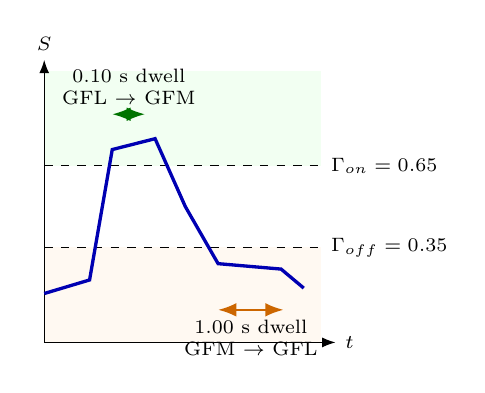
\begin{tikzpicture}[x=0.64cm,y=3.45cm,>=Latex]
\fill[green!5] (0,0.65) rectangle (5.5,1.0);
\fill[orange!5] (0,0) rectangle (5.5,0.35);
\draw[->] (0,0) -- (5.78,0) node[right,font=\scriptsize] {$t$};
\draw[->] (0,0) -- (0,1.04) node[above,font=\scriptsize] {$S$};
\draw[dashed] (0,0.65)--(5.5,0.65) node[right,font=\scriptsize] {$\Gamma_{on}=0.65$};
\draw[dashed] (0,0.35)--(5.5,0.35) node[right,font=\scriptsize] {$\Gamma_{off}=0.35$};
\draw[very thick,myblue] plot coordinates {(0,0.18) (0.9,0.23) (1.35,0.71) (2.2,0.75) (2.8,0.50) (3.45,0.29) (4.7,0.27) (5.15,0.20)};
\draw[<->,green!45!black,thick] (1.35,0.84)--(2.0,0.84);
\node[above,font=\scriptsize,align=center] at (1.68,0.84) {$0.10$ s dwell\\GFL $\rightarrow$ GFM};
\draw[<->,orange!80!black,thick] (3.45,0.12)--(4.75,0.12);
\node[below,font=\scriptsize,align=center] at (4.10,0.12) {$1.00$ s dwell\\GFM $\rightarrow$ GFL};
\end{tikzpicture}
\vspace{0.18cm}
\scriptsize
Transition is committed only after equilibrium/SSSA certification and a converged right-limit KCL solve.
\end{columns}
\end{frame}

\IfFileExists{figures/switch_ieee14_decision/run_summary_v2.tex}{% Generated by generate_ieee14_report_scalars. Do not edit.
%
% PROVENANCE. Accepted values of output/diagnostics/ieee14_gfm_lock_compare_dcreal/adaptive_250s.mat.
% Produced by run_ieee14_gfm_lock_comparison, whose option set is the
% flagship driver's plus agsi_reference=true (opt-in, post-processing only).
% This cache is NOT bit-identical to the earlier delivered artifact, and no
% such claim is made for it: the DC-link closure changed under
% NUM-2026-08-20-01, so the trajectory legitimately differs. Compare it to
% the earlier cache by outcome, never by bit-identity.
% No value here is rounded, scaled, smoothed or otherwise altered.
%
% Regenerate with:  pf_init_paths; generate_ieee14_report_scalars(result_file="output/diagnostics/ieee14_gfm_lock_compare_dcreal/adaptive_250s.mat")

\newcommand{\NewRunEnd}{250.000}
\newcommand{\NewRunVMin}{0.036855}
\newcommand{\NewRunVMax}{1.523183}
\newcommand{\NewRunFMin}{58.838795}
\newcommand{\NewRunFMax}{61.138560}
\newcommand{\NewRunSubdivision}{0}
\newcommand{\NewRunDomainRejects}{584}
\newcommand{\NewRunResidual}{$9.9596\times10^{-9}$}
\newcommand{\NewRunReclose}{159.240}
\newcommand{\NewRunRecloseStatus}{SUCCESS}
\newcommand{\NewRunSyncDV}{0.008785}
\newcommand{\NewRunSyncDF}{$6.4601\times10^{-13}$}
\newcommand{\NewRunSyncDTheta}{5.015017}
\newcommand{\NewRunFirstRelease}{25.310}
\newcommand{\NewRunReleaseOne}{25.310}
\newcommand{\NewRunReleaseTwo}{146.247}
\newcommand{\NewRunReleaseThree}{152.390}
\newcommand{\NewRunReleaseFour}{--}
\newcommand{\NewRunAugmentOne}{22.052}
\newcommand{\NewRunAugmentTwo}{51.333}
\newcommand{\NewRunAugmentThree}{53.372}
\newcommand{\NewRunAugmentFour}{148.267}
\newcommand{\NewRunNRelease}{3}
\newcommand{\NewRunNAugment}{4}
\newcommand{\NewRunGfmMax}{4}
\newcommand{\NewRunSamples}{4990}
\newcommand{\NewRunRejectedSteps}{135}
\newcommand{\NewRunTerminalF}{60.000000}
\newcommand{\NewRunTerminalVMin}{0.9667}
\newcommand{\NewRunTerminalVMax}{1.0575}
\newcommand{\NewRunStepper}{adaptive}
\newcommand{\NewRunReselection}{NO\_FEASIBLE\_SG\_ON\_ONE\_STEP}
}{}
\IfFileExists{figures/switch_ieee14_decision/comparison_macros.tex}{% Generated by generate_ieee14_gfm_lock_comparison. Do not edit.
% Every number the comparison section prints comes from here, so the prose cannot drift
% from the runs. Arm keys: adaptive, pinned_gfm1, pinned_gfm2, pinned_gfm4, locked_gfl

\newcommand{\ArmAdaptiveLabel}{adaptive}
\newcommand{\ArmAdaptiveHorizon}{250.000}
\newcommand{\ArmAdaptiveConverged}{1}
\newcommand{\ArmAdaptiveReclose}{159.2397}
\newcommand{\ArmAdaptiveGfmMax}{4}
\newcommand{\ArmAdaptiveFailure}{--}
\newcommand{\ArmAdaptiveSamples}{4990}
\newcommand{\ArmAdaptiveRejected}{135}
\newcommand{\DfAdaptiveSGtrip}{0.7587}
\newcommand{\SetAdaptiveSGtrip}{0.0041}
\newcommand{\DfAdaptiveLoadstep}{1.0035}
\newcommand{\SetAdaptiveLoadstep}{0.3753}
\newcommand{\DfAdaptiveFault}{1.1386}
\newcommand{\SetAdaptiveFault}{0.3753}
\newcommand{\DfAdaptiveLinetrip}{0.3764}
\newcommand{\SetAdaptiveLinetrip}{0.3503}
\newcommand{\DfAdaptiveRestorereclose}{1.1612}
\newcommand{\SetAdaptiveRestorereclose}{0.0130}
\newcommand{\ArmPinnedgfmOneLabel}{pinned 1 GFM}
\newcommand{\ArmPinnedgfmOneHorizon}{250.000}
\newcommand{\ArmPinnedgfmOneConverged}{1}
\newcommand{\ArmPinnedgfmOneReclose}{151.4244}
\newcommand{\ArmPinnedgfmOneGfmMax}{1}
\newcommand{\ArmPinnedgfmOneFailure}{--}
\newcommand{\ArmPinnedgfmOneSamples}{3232}
\newcommand{\ArmPinnedgfmOneRejected}{542}
\newcommand{\DfPinnedgfmOneSGtrip}{0.5312}
\newcommand{\SetPinnedgfmOneSGtrip}{0.0113}
\newcommand{\DfPinnedgfmOneLoadstep}{1.4478}
\newcommand{\SetPinnedgfmOneLoadstep}{1.2214}
\newcommand{\DfPinnedgfmOneFault}{1.4979}
\newcommand{\SetPinnedgfmOneFault}{1.2296}
\newcommand{\DfPinnedgfmOneLinetrip}{1.2325}
\newcommand{\SetPinnedgfmOneLinetrip}{1.1426}
\newcommand{\DfPinnedgfmOneRestorereclose}{1.1736}
\newcommand{\SetPinnedgfmOneRestorereclose}{0.0210}
\newcommand{\ArmPinnedgfmTwoLabel}{pinned 2 GFM}
\newcommand{\ArmPinnedgfmTwoHorizon}{250.000}
\newcommand{\ArmPinnedgfmTwoConverged}{1}
\newcommand{\ArmPinnedgfmTwoReclose}{149.9191}
\newcommand{\ArmPinnedgfmTwoGfmMax}{2}
\newcommand{\ArmPinnedgfmTwoFailure}{--}
\newcommand{\ArmPinnedgfmTwoSamples}{3183}
\newcommand{\ArmPinnedgfmTwoRejected}{321}
\newcommand{\DfPinnedgfmTwoSGtrip}{0.3489}
\newcommand{\SetPinnedgfmTwoSGtrip}{0.0001}
\newcommand{\DfPinnedgfmTwoLoadstep}{0.7839}
\newcommand{\SetPinnedgfmTwoLoadstep}{0.7123}
\newcommand{\DfPinnedgfmTwoFault}{0.8255}
\newcommand{\SetPinnedgfmTwoFault}{0.7126}
\newcommand{\DfPinnedgfmTwoLinetrip}{0.7135}
\newcommand{\SetPinnedgfmTwoLinetrip}{0.6422}
\newcommand{\DfPinnedgfmTwoRestorereclose}{0.6634}
\newcommand{\SetPinnedgfmTwoRestorereclose}{0.0209}
\newcommand{\ArmPinnedgfmFourLabel}{pinned 4 GFM}
\newcommand{\ArmPinnedgfmFourHorizon}{25.491}
\newcommand{\ArmPinnedgfmFourConverged}{0}
\newcommand{\ArmPinnedgfmFourReclose}{--}
\newcommand{\ArmPinnedgfmFourGfmMax}{4}
\newcommand{\ArmPinnedgfmFourFailure}{\texttt{adaptiveDtMin}}
\newcommand{\ArmPinnedgfmFourSamples}{819}
\newcommand{\ArmPinnedgfmFourRejected}{449}
\newcommand{\DfPinnedgfmFourSGtrip}{0.9898}
\newcommand{\SetPinnedgfmFourSGtrip}{--}
\newcommand{\DfPinnedgfmFourLoadstep}{--}
\newcommand{\SetPinnedgfmFourLoadstep}{--}
\newcommand{\DfPinnedgfmFourFault}{--}
\newcommand{\SetPinnedgfmFourFault}{--}
\newcommand{\DfPinnedgfmFourLinetrip}{--}
\newcommand{\SetPinnedgfmFourLinetrip}{--}
\newcommand{\DfPinnedgfmFourRestorereclose}{--}
\newcommand{\SetPinnedgfmFourRestorereclose}{--}
\newcommand{\ArmLockedgflLabel}{locked GFL}
\newcommand{\ArmLockedgflHorizon}{20.000}
\newcommand{\ArmLockedgflConverged}{0}
\newcommand{\ArmLockedgflReclose}{--}
\newcommand{\ArmLockedgflGfmMax}{0}
\newcommand{\ArmLockedgflFailure}{\texttt{noVoltageFormingSource}}
\newcommand{\ArmLockedgflSamples}{43}
\newcommand{\ArmLockedgflRejected}{0}
\newcommand{\DfLockedgflSGtrip}{--}
\newcommand{\SetLockedgflSGtrip}{--}
\newcommand{\DfLockedgflLoadstep}{--}
\newcommand{\SetLockedgflLoadstep}{--}
\newcommand{\DfLockedgflFault}{--}
\newcommand{\SetLockedgflFault}{--}
\newcommand{\DfLockedgflLinetrip}{--}
\newcommand{\SetLockedgflLinetrip}{--}
\newcommand{\DfLockedgflRestorereclose}{--}
\newcommand{\SetLockedgflRestorereclose}{--}
\newcommand{\CommonWindowPinnedgfmOneBitIdentical}{1}
\newcommand{\CommonWindowPinnedgfmOneSamples}{42}
\newcommand{\CommonWindowPinnedgfmTwoBitIdentical}{1}
\newcommand{\CommonWindowPinnedgfmTwoSamples}{42}
\newcommand{\CommonWindowPinnedgfmFourBitIdentical}{1}
\newcommand{\CommonWindowPinnedgfmFourSamples}{42}
\newcommand{\CommonWindowLockedgflBitIdentical}{1}
\newcommand{\CommonWindowLockedgflSamples}{42}
\newcommand{\CommonWindowSplit}{20.000}
\newcommand{\CommonWindowAllBitIdentical}{1}
\newcommand{\CandTotal}{15}
\newcommand{\CandReady}{7}
\newcommand{\CandBestSet}{IBR3+IBR6}
\newcommand{\CandBestN}{2}
\newcommand{\CandBestOmega}{-0.56814}
\newcommand{\CandBestSingleOmega}{-0.32801}
\newcommand{\CandFullOmega}{-0.48291}
\newcommand{\CandReadyNOne}{4}
\newcommand{\CandTotalNOne}{4}
\newcommand{\CandReadyNTwo}{2}
\newcommand{\CandTotalNTwo}{6}
\newcommand{\CandReadyNThree}{0}
\newcommand{\CandTotalNThree}{4}
\newcommand{\CandReadyNFour}{1}
\newcommand{\CandTotalNFour}{1}
}{}
\section{Results}
\begin{frame}{Result 1: GFM Candidate Screening}
\begin{columns}[c,onlytextwidth]
\column{0.56\textwidth}
\scriptsize
\begin{tabular}{cll}
\toprule
GFM count & Candidate & Outcome \\
\midrule
1 & any single IBR & admissible \\
2 & IBR1 + IBR3 & admissible \\
2 & \textbf{IBR2 + IBR3} & \textbf{best margin} \\
2 & other pairs & rejected \\
3 & any triple & rejected \\
4 & all four IBRs & admissible \\
\bottomrule
\end{tabular}
\vspace{0.32cm}
\begin{block}{Observed property}
Admissibility is \textbf{non-monotonic} in the number of grid-forming converters.
\end{block}
\column{0.40\textwidth}
\centering
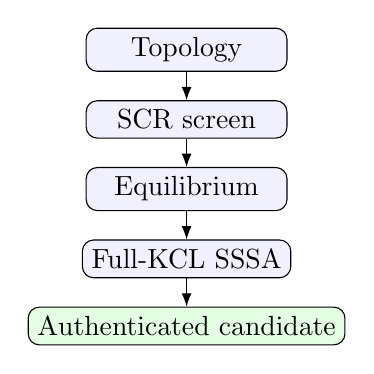
\begin{tikzpicture}[node distance=3.6mm,>=Latex]
\node[draw,rounded corners,fill=blue!6,minimum width=2.55cm] (a) {Topology};
\node[draw,rounded corners,fill=blue!6,below=of a,minimum width=2.55cm] (b) {SCR screen};
\node[draw,rounded corners,fill=blue!6,below=of b,minimum width=2.55cm] (c) {Equilibrium};
\node[draw,rounded corners,fill=blue!6,below=of c,minimum width=2.55cm] (d) {Full-KCL SSSA};
\node[draw,rounded corners,fill=green!10,below=of d,minimum width=2.55cm] (e) {Authenticated candidate};
\draw[->] (a)--(b); \draw[->] (b)--(c); \draw[->] (c)--(d); \draw[->] (d)--(e);
\end{tikzpicture}
\vspace{0.18cm}
\footnotesize
The GFM set is computed from the current network condition; converter count alone does not determine admissibility.
\end{columns}
\end{frame}
\begin{frame}{Result 2: Disturbance Scenario}
\begin{center}
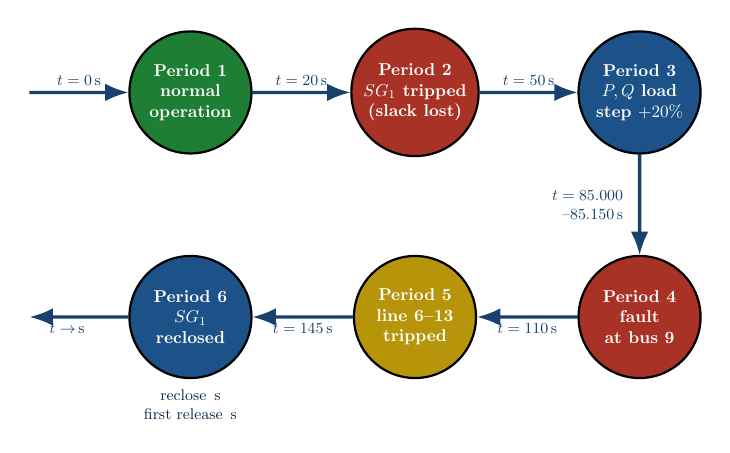
\begin{tikzpicture}[
  scale=0.62,transform shape,
  per/.style={circle,draw,thick,minimum size=2.5cm,inner sep=2pt,
    align=center,text=white,font=\bfseries},
  tlbl/.style={font=\small},
  tlab/.style={midway,above,font=\small},
  tlabb/.style={midway,below,font=\small},
  arr/.style={-{Latex[length=3mm]},very thick,color=pblue!80!black}]
\node[per,fill=pgreen] (p1) at (0,0)     {Period 1\\ normal\\ operation};
\node[per,fill=pred]   (p2) at (4.6,0)   {Period 2\\ $SG_1$ tripped\\ (slack lost)};
\node[per,fill=pblue]  (p3) at (9.2,0)   {Period 3\\ $P,Q$ load\\ step $+20\%$};
\node[per,fill=pred]   (p4) at (9.2,-4.6){Period 4\\ fault\\ at bus 9};
\node[per,fill=pyellow](p5) at (4.6,-4.6){Period 5\\ line 6--13\\ tripped};
\node[per,fill=pblue]  (p6) at (0,-4.6)  {Period 6\\ $SG_1$\\ reclosed};
\draw[arr] (-3.3,0) -- node[tlab]{$t=0$\,s} (p1);
\draw[arr] (p1) -- node[tlab]{$t=20$\,s} (p2);
\draw[arr] (p2) -- node[tlab]{$t=50$\,s} (p3);
\draw[arr] (p3) -- node[font=\small,left=2mm,pos=0.5,align=right]{$t=85.000$\\--$85.150$\,s} (p4);
\draw[arr] (p4) -- node[tlabb]{$t=110$\,s} (p5);
\draw[arr] (p5) -- node[tlabb]{$t=145$\,s} (p6);
\draw[arr] (p6) -- node[tlabb,pos=0.62]{$t\to\NewRunEnd$\,s} ++(-3.3,0);
\node[tlbl,below=3pt of p6,align=center,text=pnavy]
  {reclose $\NewRunReclose$\,s\\ first release $\NewRunFirstRelease$\,s};
\end{tikzpicture}
\end{center}
\vspace{-0.15em}
\scriptsize
Green: undisturbed; red: source loss or fault; yellow: topology change; blue: restorative action. Scheduled times are case-defined; reclose and release times are read from the accepted event log.
\end{frame}

\begin{frame}{Result 3: Electrical Response}
\centering
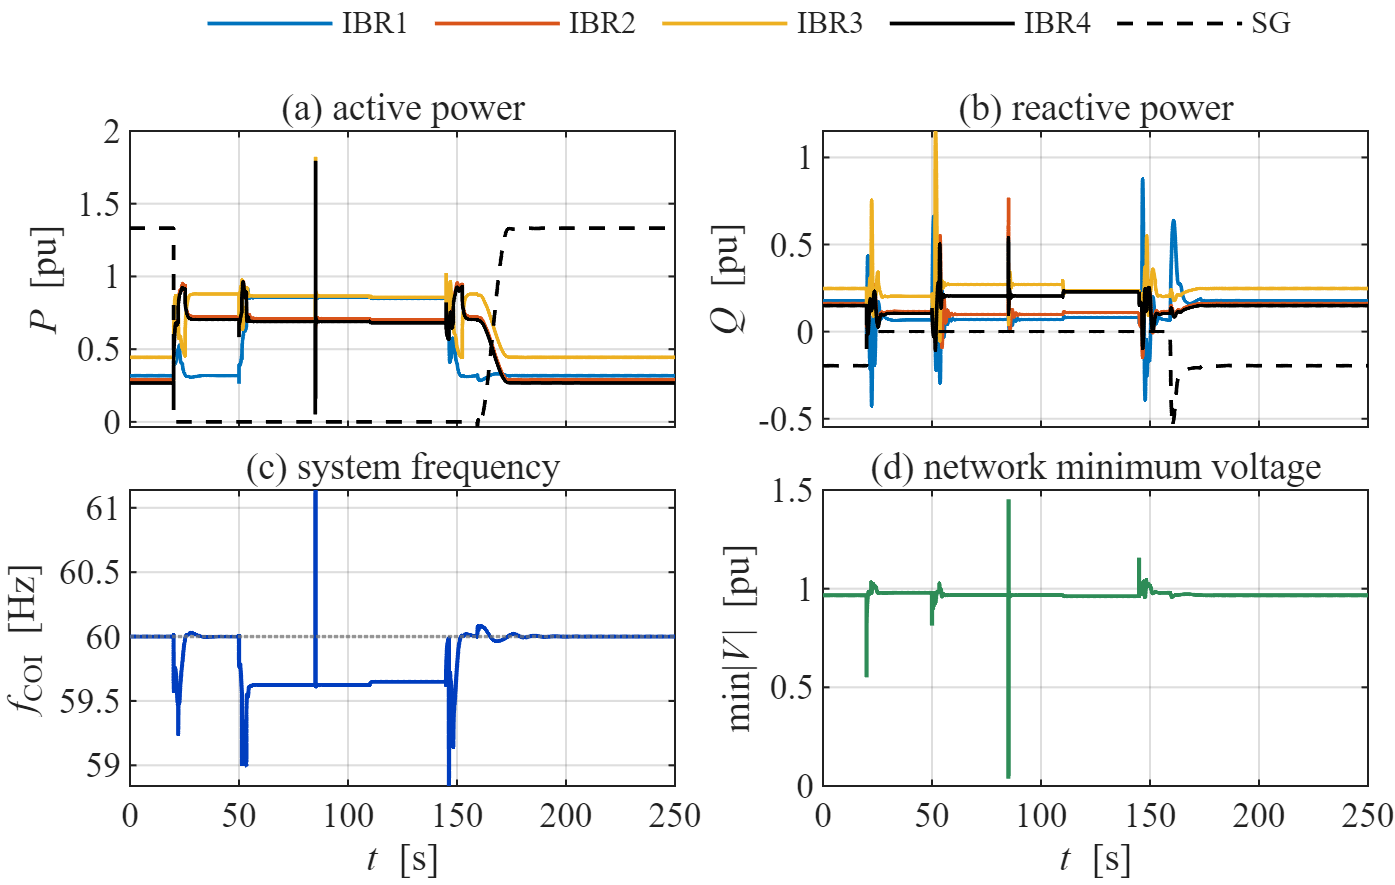
\includegraphics[width=0.97\textwidth,height=0.76\textheight,keepaspectratio]{figures/presentation_pf_sssa_ts_gfm/slide_electrical_v4.png}
\vspace{0.08cm}
\scriptsize
System active/reactive power, COI frequency, and minimum bus voltage over the complete $250$ s chronology.
\end{frame}
\begin{frame}{Result 4: Converter Response under Different Policies}
\centering
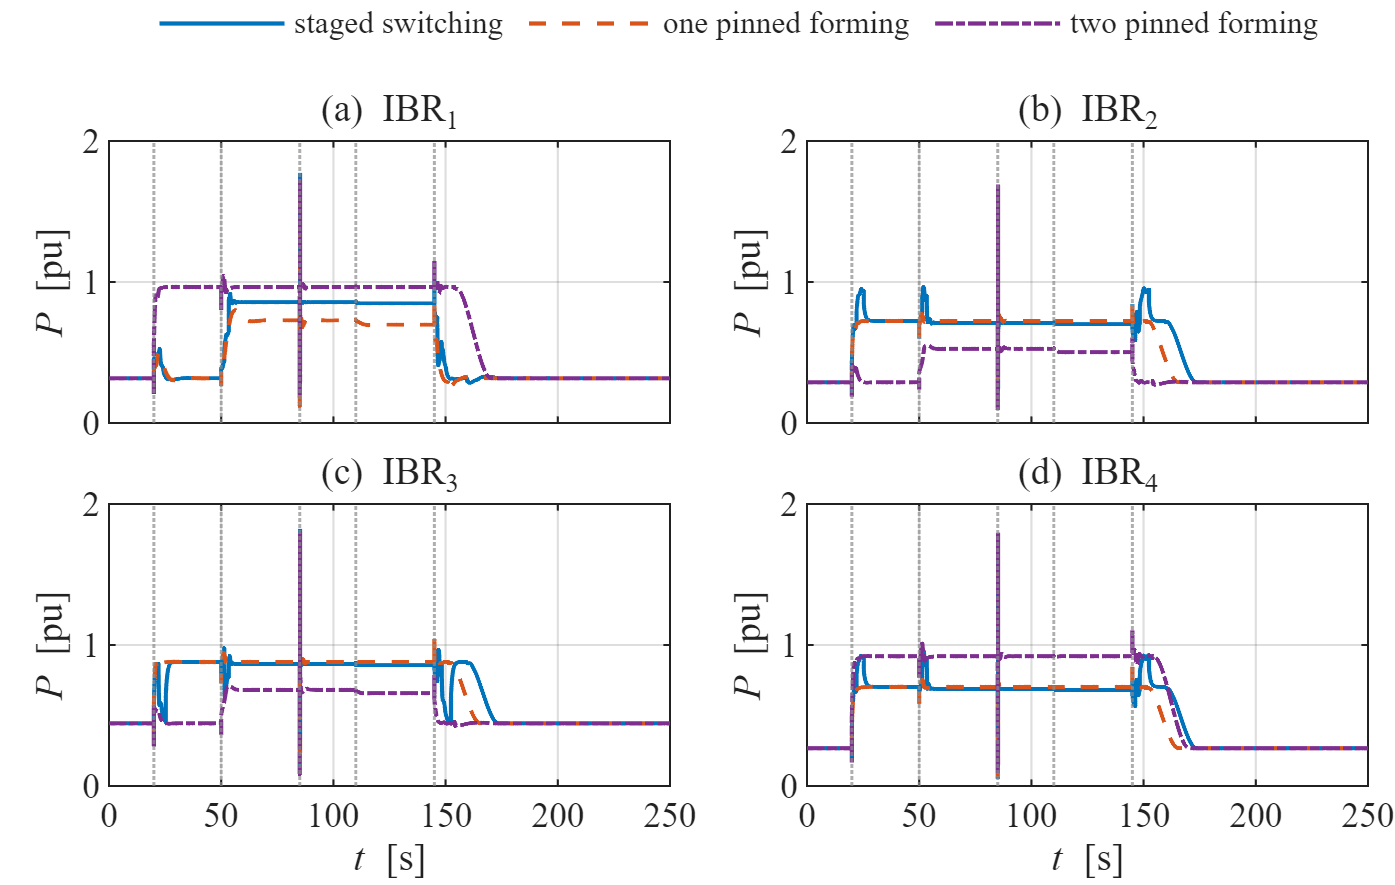
\includegraphics[width=0.97\textwidth,height=0.76\textheight,keepaspectratio]{figures/presentation_pf_sssa_ts_gfm/slide_per_converter_v4.png}
\vspace{0.08cm}
\scriptsize
IBR1--IBR4 active-power response: staged switching (solid), one pinned GFM (dashed), and two pinned GFMs (dash-dot).
\end{frame}

\section{Conclusion}
\begin{frame}{Conclusion and Key Findings}
\begin{columns}[c,onlytextwidth]
\column{0.56\textwidth}
\footnotesize
\begin{itemize}
  \item PF, SSSA, and TS are linked through one nonlinear SG/IBR network model.
  \item After SG1 is disconnected, at least one voltage-forming IBR is required for the islanded trajectory to continue.
  \item GFM admissibility is configuration-dependent and non-monotonic in converter count.
  \item Staged switching reaches the full $250$ s chronology and returns all IBRs to GFL operation after SG recovery.
\end{itemize}
\column{0.40\textwidth}
\footnotesize
\begin{block}{Comparative outcome}
\begin{itemize}
  \item \textbf{Locked GFL:} stops at $20$ s; no forming source.
  \item \textbf{1--2 pinned GFMs:} reach $250$ s; reclose succeeds.
  \item \textbf{4 pinned GFMs:} nonlinear failure at $25.485$ s.
  \item \textbf{Staged switching:} $250$ s with full hand-back.
\end{itemize}
\end{block}
\end{columns}
\vspace{0.12cm}
\footnotesize
\textbf{Scope of claim:} the staged policy is not claimed to minimize every transient peak; its benefit here is adaptive reference support across the complete disturbance chronology.
\end{frame}

\end{document}
